\documentclass[10pt, oneside]{article} 
\usepackage{amsmath, amsthm, amssymb, calrsfs, wasysym, verbatim, bbm, color, graphics, geometry}
\usepackage[colorlinks=true, linkcolor=blue, urlcolor=blue, citecolor=blue]{hyperref} % Customize hyperref
\usepackage{csquotes} % For the \enquote command
\usepackage[dvipsnames]{xcolor} % For colored text
\usepackage{tcolorbox} % For custom boxes
\usepackage{multicol}

\usepackage{tikz}
\usetikzlibrary{arrows.meta, decorations.markings}
\tikzset{
    vector/.style={thick,->},
    angle/.style={thin, red},
    angle label/.style={font=\small, red},
}

\usepackage{multicol}

\newtheorem{theorem}{Theorem}
\newtheorem*{theorem*}{Theorem}

\theoremstyle{remark}
\newtheorem*{own_abstract}{Abstract}
\newtheorem*{proofsketch}{Proof Sketch}

% Define the new command for boxed notes
\newcommand{\myBoxedNote}[1]{%
  \hspace{40pt} \boxed{\textbf{Sidenote: } #1}%
}

% counter for definitions
\newcounter{definition}
% Define the new environment for definitions
\newtcolorbox{myDef}[1][]{
  colback=gray!10!white, colframe=gray!80!black, fonttitle=\bfseries,
  title=Definition \thedefinition\ifstrempty{#1}{}{ (#1)},
  rounded corners, before upper={\stepcounter{definition}}
}

% counter for theorems
\newcounter{theoremCounter}

% define the new environment for theorems
\newtcolorbox{myTheo}[1][]{
  colback=red!10!white, colframe=red!50!black, fonttitle=\bfseries,
  title=Theorem \thetheoremCounter\ifstrempty{#1}{}{ (#1)},
  rounded corners, before upper={\stepcounter{theoremCounter}}
}

\newcounter{claimCounter}
\newtcolorbox{myClaim}[1][]{
  colback=white, colframe=black, fonttitle=\bfseries,
  title=Claim \theclaimCounter\ifstrempty{#1}{}{ (#1)},
  rounded corners, before upper={\stepcounter{claimCounter}}
}

\geometry{tmargin=.75in, bmargin=.75in, lmargin=.75in, rmargin = .75in}  

\newtheorem{thm}{Theorem}
\newtheorem{defn}{Definition}
\newtheorem{conv}{Convention}
\newtheorem{rem}{Remark}
\newtheorem{lem}{Lemma}
\newtheorem{cor}{Corollary}

\title{Base information about the Learning Unit}
\author{Fabian Stiewe}
\date{Academic Year 2024-2025}

\begin{document}

\maketitle
\tableofcontents

\newpage

\section{School and Year}
This learning unit is designed for the 4th year of the \textbf{ITT - Istituto Tecnico Tecnologico}. It will be taught at the beginning of the academic year as an introduction to \enquote{efficient} algorithm. After this unit, a Learning Unit like \textit{Data Structures (Stacks, Queues, Heap, etc.)} could be taught to extend the theory and practice knowledge of the students.

\section{Materials}
For the theory part the students need a notebook, pen and a mobile device to use the platform \href{https://tcs.uni-frankfurt.de/algo-learn-testing/refs_heads_feat-bubbleSort/en}{algo learn} and \href{https://kahoot.it/}{Kahoot!}. For the practice part we will go to the laboratory, where the students will have access to a computer with their preferred programming language installed.

\section{Topics to be covered}
The main topic is the connection between \textbf{theoretical computer science} and \textbf{programming}, inside this huge field we will focus on the following topics:
\begin{itemize}
  \item Sorting algorithms
  \begin{itemize}
    \item Bubble sort
    \item Selection sort
    \item Merge sort
    \item Sorting on presorted data
  \end{itemize}    
  \item Searching algorithms
  \begin{itemize}
    \item Linear search
    \item Binary search
    \item Hash tables
  \end{itemize}
\end{itemize}
\textbf{Since the students will also implement every algorithm and use them in a real application, they will also learn how to use a programming language to solve problems.} 

\textbf{9 weeks} seems to be a lot, but the students will also have to implement the algorithms in the laboratory, which will take a lot of time and will improve programming skills too. So it is a combined unit of theoretical computer science and programming.

\subsection{Objectives Sorting Algorithms}

\subsubsection{Bubble Sort}
The students should understand how the \textbf{bubble sort} algorithm works and be able to implement it in their preferred programming language. They should also be able to analyze the time complexity \textit{(not with big-O notation)} of the algorithm and understand why it is not efficient for large data sets.

\subsubsection{Selection Sort}
The students should understand how the \textbf{selection sort} algorithm works and be able to implement it in their preferred programming language. They should also be able to analyze the time complexity \textit{(not with big-O notation)} of the algorithm and understand why it is not efficient for large data sets.

\subsubsection{Merge Sort}
The students should understand how the \textbf{merge sort} algorithm works and be able to implement it in their preferred programming language. A time complexity is \textbf{not} required, but the students should understand that it is more efficient than bubble sort and selection sort.

\subsubsection{Sorting on Presorted Data}
Given different data sets, the students should be able to choose the best sorting algorithm for each data set. They should also be able to explain why a specific sorting algorithm is better for a specific data set.

In example: If the data set is already sorted, except for $k$ elements, which sorting algorithm should be used?

\subsection{Objectives Searching Algorithms}

\subsubsection{Linear Search}
The students should understand how the \textbf{linear search} algorithm works and be able to implement it in their preferred programming language. They should also be able to analyze the time complexity \textit{(not with big-O notation)} of the algorithm and understand why it is not efficient for large data sets.

\subsubsection{Binary Search}
The students should understand how the \textbf{binary search} algorithm works and be able to implement it in their preferred programming language. They should also be able to analyze the time complexity \textit{(not with big-O notation)} of the algorithm and understand why it is more efficient than linear search.

\subsubsection{Hash Tables}
The students should understand how \textbf{hash tables} work and be able to use them in their preferred programming language. They should understand why it is efficient for searching and inserting elements and be able to explain why it is more efficient than binary search (in special cases).

\subsection{Summarize Objectives}
The students will be able to \textbf{implement} different sorting and searching algorithms and will see cases from real application where those algorithms are used.

\section{Prerequisites}
There are no formal prerequisites for this learning unit. However, it is recommended that students have a basic understanding of the following topics:
\begin{itemize}
  \item Basic programming concepts
  \begin{itemize}
    \item The programming language does not matter, each student can use the language they are most comfortable with
    \item Variables, loops, functions, arrays, etc. should be known
  \end{itemize}
  \item Basic mathematics concepts
  \begin{itemize}
    \item Basic algebra
    \item $\log$ function
    \item Very basic probability (there won't be a proof for hash tables, but it helps to understand the concept)
  \end{itemize}
\end{itemize}

\section{Time plan for the Learning Unit}
The learning unit will take 9 weeks (6 hours a week). Each week will be divided into two parts: \textbf{theory} (2h) and \textbf{practice} (4h). The theory part will be taught first, and the practice part will be taught (in the laboratory) in the second half of the week. During the practice part, the students will get a problem (different difficulties) and should implement a solution using the algorithms they learned in the theory part, adapted to the corresponding problem (logical thinking).

\subsection{Week 1: Bubble Sort}
Using a presentation, the students will get taught how the bubble sort algorithm works. They will also get some examples and the \enquote{Pseudocode} of the algorithm. 

The students will play two little games, first they will sort each other by height using the bubble sort algorithm. Second they will learn the algorithm (\textit{also at home}) using the platform \href{https://tcs.uni-frankfurt.de/algo-learn-testing/refs_heads_feat-bubbleSort/en
}{algo learn} \textbf{(Only the part for sorting algorithms)}.

In the laboratory, the students will get following problems and should implement a solution using the bubble sort algorithm.

\subsubsection*{Problem for the laboratory}
\begin{tcolorbox}
  To start the course the students will get a simple problem: Given an array of integers, sort the array using the bubble sort algorithm. The array should be sorted in ascending order. 
  
  \vspace{1em}
  
  Additional keep track of how many swaps are needed to sort the array.
  
  \vspace{1em}
  
  For those who are fast: Given an array of tuples, the first entry is a string and the second entry is an integer. First sort the array by the integer in ascending order, then sort the array by the string in descending order.
\end{tcolorbox}

\subsection{Week 2: Selection Sort}
Using a presentation, the students will get taught how the selection sort algorithm works. They will also get some examples and the \enquote{Pseudocode} of the algorithm. Also, an application example will be shown, quite similar to the problem for the laboratory. 

They will again play two little games,  and using the platform \href{https://tcs.uni-frankfurt.de/algo-learn-testing/refs_heads_feat-bubbleSort/en
}{algo learn} to learn the \textbf{selection sort} algorithm. 

\subsubsection*{Problem for the laboratory}
\begin{tcolorbox}
  You are given an array of strings \texttt{names}, and an array \texttt{heights} that consists of distinct positive integers. Both arrays are of length $n$. For each index $i$, \texttt{names}$[i]$ and \texttt{heights}$[i]$ denote the name and height of the $i$th person. Return \texttt{names} sorted in descending order by the people's heights.

  \vspace{1em}

  Given a list of numbers $A$ with $a_i \in \mathbb{Z}$, decide if there is a pair of indices $(i, j)$ such that $a_i + a_j = 0$. Extend this case to a triplet $(i, j, k)$ such that $a_i + a_j + a_k = 0$.

  \vspace{1em}
  Even a little more complicated: Decide if there is such a pair of indices $(i, j)$ such that $a_i + a_j = 0$ and $i + j = |a_i - a_j|$.
\end{tcolorbox}
The first problem should be solved using the selection sort algorithm, the second and third problem are more logical problems, which don't necessarily need the selection sort algorithm.

\subsection{Week 3: Merge Sort}
Again using a presentation and the following YouTube video: \href{https://www.youtube.com/watch?v=ZRPoEKHXTJg}{Merge Sort Animations}. The students will get taught how the merge sort algorithm works. They will also get some examples and the \enquote{Pseudocode} of the algorithm.

They will again use the platform \href{https://tcs.uni-frankfurt.de/algo-learn-testing/refs_heads_feat-bubbleSort/en
}{algo learn} to learn the \textbf{merge sort} algorithm and if there is time left, they will play a little game to sort each other by height again using the merge sort algorithm.

\subsubsection*{Problem for the laboratory}
\begin{tcolorbox}
  You are given an array of integers. Sort the array using the merge sort algorithm. The array should be sorted in ascending order. 

  \vspace{1em}
  
  Count how many inversions are in the array. An inversion is a pair of indices $(i, j)$ such that $i < j$ and $a[i] > a[j]$.

  \vspace{1em}

  Given two sequences of integers in the $xy$-plane, namely $p_1, \dots, p_n$ in $y=0$ and $q_1, \dots, q_n$ in $y=1$. We create $n$ lines, each line connects $(p_i, 0)$ and $(q_i, 1)$. Return the number of crossing lines.
  \begin{center}
    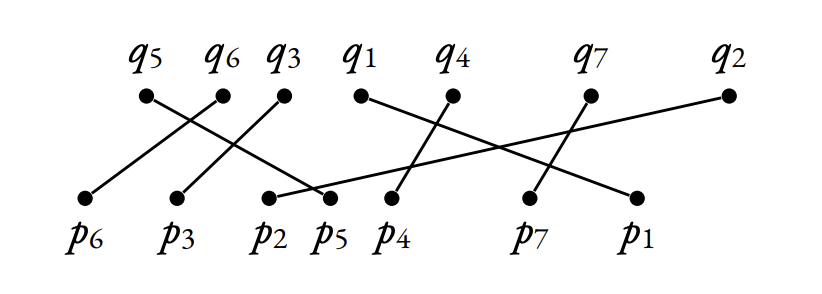
\includegraphics[width=0.5\textwidth]{MergeSortProblem.png}
  \end{center}
  Example with $n=7$ and $8$ crossing lines. As input, you get the two arrays $p$ and $q$, where $p[i]$ and $q[i]$ are the $x$-coordinates of the points $p_i$ and $q_i$. You can assume that no two $x$-coordinates are the same.
    

\end{tcolorbox}

\subsection{Week 4: Sorting on Presorted Data}
Will be created during the course.

\subsection{Week 5: Recap and evaluation of the sorting algorithms}
Will be created during the course. There will be more programming challenges, to show the connection between theoretical computer science and programming. Logical thinking of each student will be challenged.

I explore following problem on 05.12.: \href{https://adventofcode.com/2024/day/5}{AOC day 5}. Part 1 and Part 2 are interesting, because they are related to sorting algorithms and show a connection to a real application (even though artificially created). The students will get enough hints to solve the problem. 

\subsection{Week 6: Linear Search}
Will be created during the course.

\subsection{Week 7: Binary Search}
Will be created during the course.

\subsection{Week 8: Hash Tables}
Will be created during the course.

\subsection{Week 9: Recap and evaluation of the searching (and sorting) algorithms}
Will be created during the course.

\section{Support for Diverse Learning Needs}
If a student is learning \textit{slower} than the others, the student will get additional help. There are most of the time many diverse videos and online sources, which can help the student to understand the topic. During the laboratory, the student will get additional help from the teacher, by getting hints and tips to solve the problem.

\section{Evaluation}
\subsection{Outline}
The main part of the evaluation will be the programming during the laboratory. The students will get a problem and should implement a solution using the algorithms they learned in the theory part. The implementation should be correct and efficient, or at least the students should be able to explain why their implementation is not efficient. \textbf{This will make approximately 60\% of the final grade.}

Above that, the Mini-Tests (in week 5 and 9) will be used to evaluate the understanding of the algorithms. The students should be able to explain how the algorithms work and why they are efficient or not efficient. 

\begin{tcolorbox}
  I would like to use the platform \href{https://tcs.uni-frankfurt.de/algo-learn-testing/refs_heads_feat-bubbleSort/en}{algo learn} for evaluation. It is \textbf{planned} as a feature in the future, such that students login in, and the teacher gets the learning data.
\end{tcolorbox}

\subsection{Mini-Test Week 5}
\subsubsection{No. 1 - Bubble Sort}
You are given the following list of numbers: 
\begin{align*}
  [5, 3, 8, 2, 1, 4, 7, 6]
\end{align*}
\begin{enumerate}
  \item Sort the list using the bubble sort algorithm. Write down the list after each iteration. ($5$P)
  \item What is the time complexity of the bubble sort algorithm? ($2$P)
  \item Why is the bubble sort algorithm not efficient for large data sets? ($2$P)
  \item What is the best case time complexity of the bubble sort algorithm? ($1$P)
\end{enumerate}

\subsubsection{No. 2 - Selection Sort}
You are given the following list of numbers:
\begin{align*}
  [12, 3, 5, 7, 1, 9, 4, 6]
\end{align*}
\begin{enumerate}
  \item Please sort the list using the selection sort algorithm. Write down the list after each iteration. ($5$P)
  \item Explain the difference between the bubble sort and the selection sort algorithm. ($3$P)
\end{enumerate}

\subsubsection{No. 3 - Merge Sort}
You are given the following list of numbers:
\begin{align*}
  [8, 2, 4, 6, 3, 1, 5, 7]
\end{align*}
\begin{enumerate}
  \item Please sort the list using the merge sort algorithm. Write down the list after each iteration. ($4$P)
  \item What is the time complexity of the merge sort algorithm? ($2$P)
  \item Why is the merge sort algorithm more efficient than the bubble sort and selection sort algorithm? ($2$P)
\end{enumerate}

\subsubsection{No. 4 - Sorting on Presorted Data}
Given will be the following list of numbers, choose the best sorting algorithm for each list and explain why you choose this algorithm. (each $3$P)
\begin{enumerate}
  \item $[1, 2, 3, 4, 5, 6, 7, 8]$
  \item $[8, 7, 6, 5, 4, 3, 2, 1]$
  \item $[8, 2, 4, 6, 3, 1, 5, 7]$
\end{enumerate}

\subsection{Mini-Test Week 9}
This will be created during the course.


\end{document}